\documentclass[11pt]{exam}
%\usepackage{euscript}

\usepackage{amsmath}
\usepackage{amsthm}
\usepackage{amssymb}
\usepackage{epsfig}
\usepackage{xspace}
\usepackage{color}
\usepackage{url}
\usepackage{subfig}
\usepackage{float}
\usepackage{array}
\usepackage{graphicx}
\graphicspath{ {images/} }
%%%%%%%  For drawing trees  %%%%%%%%%
\usepackage{tikz}
\usetikzlibrary{calc, shapes, backgrounds}

%%%%%%%%%%%%%%%%%%%%%%%%%%%%%%%%%
\setlength{\textheight}{9in}
\setlength{\topmargin}{-0.600in}
\setlength{\headheight}{0.2in}
\setlength{\headsep}{0.250in}
\setlength{\footskip}{0.5in}
\flushbottom
\setlength{\textwidth}{6.5in}
\setlength{\oddsidemargin}{0in}
\setlength{\evensidemargin}{0in}
\setlength{\columnsep}{2pc}
\setlength{\parindent}{1em}
%%%%%%%%%%%%%%%%%%%%%%%%%%%%%%%%%


\newcommand{\eps}{\varepsilon}

\renewcommand{\c}[1]{\ensuremath{\EuScript{#1}}}
\renewcommand{\b}[1]{\ensuremath{\mathbb{#1}}}
\newcommand{\s}[1]{\textsf{#1}}
\newcommand{\tb}[1]{\textbf{#1}}

\newcommand{\E}{\textbf{\textsf{E}}}
\renewcommand{\Pr}{\textbf{\textsf{Pr}}}
%\footnote{\s{CS 6140  Data Mining; \;\; Spring 2015 \hfill
%Instructor: Jeff M. Phillips, University of Utah}
%}

%\title{CS 6140 Data Mining Project Final Report}
%\author{Padmashree Teeka (u0880562), Roshani Nagmote (u0941394), Anirudh Narasimhamurthy (u0941400)}

\begin{document}

\begingroup
\fontsize{14pt}{16pt}\selectfont
\begin{center}  
	CS 6140 Data Mining Project Final Report \\
	
\end{center}  
\endgroup
\textbf{\underline{Comparing performances of different clustering techniques on network datasets. }} \\

\section{Team Members}

\begin{itemize}
	\item[]
	
	\begin{itemize}
		\item Padmashree Teeka (u0880562)
		\item Roshani Nagmote (u0941394)
		\item Anirudh Narasimhamurthy (u0941400)
	\end{itemize}

\end{itemize}


\section{ Problem and Motivation}

\begin{itemize}
\item[]

In this digital age of Facebook, Amazon, Twitter, Wikipedia , Pinterest, Yelp and other numerous online social networks, finding groups of individuals or objects that are similar to each other but different from other indivduals in other groups can be \textbf{profitable} for companies, intellectually satisfying for reserachers or in case of a grad student both of it, as it could potentially prove to be profitable for a project submission and as well as one gets to understand better the concept of \textbf{"clustering"} !

\item[] Clustering such large networks is a challenging task in itself given the volume and size which we are dealing with and exploring them could lead to several interesting results.

\item[] Comparing the different cluster formulations and finding the clustering formulation\ technique which works best for a problem was our motivation in taking up this project.

\end{itemize}

\section{Key Idea}

\begin{itemize}

\item [] Given that there are several clustering formulations out there in the wild, if only we had a fairy or an oracle throwing out \textbf{the clustering formulation that would be best suited for our given problem}, whenever we needed, things would have been great. But sadly since there seems to be no such fairy existing, we thought why don't we learn and get to play the fairy.

\item[] The concept of finding people who could potentially be part of particular groups based on their connections or friendhsip is an interesting one and has effectively been used by several companies online to attract customers.

\item[] Since we were interested in exploring the different clustering formulations on large networks, we decided to take up three such techniques and compare their performances on these networks. The clustering techniques which we explored are :
	\begin{itemize}
		\item  \textbf{Assignment based clustering (K-means)}
		\item \textbf{Hierarchical/ Agglomerative Clustering}
		\item \textbf{Spectral Clustering}
	\end{itemize}	


\item[] Given that we were trying to explore large networks which are generally represented by nodes and edges, the geometry of the data makes it likely that spectral clustering would perform well among the three techniques which we have taken into consideration.

\end{itemize}


\section{Data exploration and Processing}

\begin{itemize}
\item []
Given that the motivation and key idea has provided a neat segue, we describe in this section the data with which we played with. We looked at the different datasets in the Stanford Large Network Dataset Collection\cite{one} and found the \textbf{LiveJournal dataset} to be an interesting one to explore.

\subsection{ Dataset information }

Our dataset basically represents the friendship network with no additional information about the users profile or other features. Since this was part of research data and it was being obtained from social network, the data is also in anonymized format. Live journal allows users to form a group in which other members can join. The concept of groups is directly related to the concept of "Clustering"

\subsection{Data processing}

 The dataset format was basically a list of \textbf{From nodes} and \textbf{To Nodes}  along with a header information. The nodes represent the \textbf{Users} and edges represent the connection between two users in the online blogging community or in social networking terms "Friends" or "Followers/Following". Like with most of the social networks the edge represents an undirected edge.

 The data was readily available and we did not have to do much of data munging or cleaning apart from handling the header information in the code. The dataset however comprised of nodes and edges which were in the range of millions. To be exact, the number of nodes and edges were :

\begin{table}[h]
	\centering
	\begin{tabular}{|c|c| c|}
		\hline
		\textbf{Dataset}  & \textbf{Nodes} & \textbf{Edges} \\
		\hline
		Live Journal & 3,997,962 & 34,681,189\\
		\hline
 \end{tabular}
 \caption{Datasets and no of nodes and edges}
 \label{t2}
\end{table}
The exact specifics of how we processed and stored our data would be explained in the later sections as we had variations for each of the clustering techniques.

%\end{itemize}


\subsection{Data simulation}

We did in the course of running our experiments on the dataset, face issues with scalability. We simulated a smaller data set by combining few functions from the \textbf{networkx and numpy} packages in Python and created the list of edges in the network, which maintained consistency as per our original data set representation. Basically the code created adjacency lists of specified length, where length corresponds to the number of nodes in the network. We then handled how this data was to be written in the same format in which our original dataset was and ran our experiments on the smaller dataset.

The results produced by the simulated data sets are mentioned in the later sections.

\subsection{ Network datasets used for experiments}

Apart from the large Live Journal dataset, we also wanted to compare the performances across smaller and medium sized networks. One of the smaller datasets was obtained by simulation descibed in the above section. The following are the networks which we have considered while performing our experiments :


\begin{table}[h]
	\centering
	\begin{tabular}{|c|c| c| c|}
		\hline
		\textbf{Dataset}  & \textbf{Nodes} & \textbf{Edges} & Size-scale\\
		\hline
		Random & 50 & 151 & Tiny\\
		\hline
		GNutella & 6301 & 20,777 & Small\\
		\hline
		DBLP & 317,080 & 1,049,866 & Small\\
		\hline
	\end{tabular}
	\caption{Experimental Datasets with number of nodes and edges}
	\label{t2}
\end{table}

The datasets GNutella represents a peer to peer network and the DBLP dataset also represents a quasi social network graph. Since these two datasets are closely related in real world meaning and in data with our main dataset, we considered them for our experiments for lower sized datasets.

\end{itemize}

\section{ Decription of the three clustering formulations}

\subsection{Spectral Clustering}

	 Given our data is a network of nodes or in other words a graph, our intuition was to start with a clustering technique which would be coherent match to the problem. Spectral Clustering is "top-down" clustering where we start with one big cluster and then go on and divide the big cluster into smaller and smaller clusters.\\
	
	 With respect to our dataset this primarily implies we start with all the users being part of one large group or the social network and then we are interested in finding smaller groups which would have similar people. This idea of groups can be extended to any social networks.\\
	
	\textbf{\underline{Programming Platform Used:  MATLAB}} 
	
	\subsubsection{Data Storage}
	\begin{itemize}
		\item 
		 The first step was to get the data loaded into matrix and since the data was entirely consisting of nodes and edges, constructing the adjacency matrix was the first logical step.
		 
		 \item We loaded the tab separated data file into a matrix in MATLAB using the 'Load()' function and we were able to get the entire data loaded into a matrix. 
		 
		 \item This was also one of our reasons for going with MATLAB for the implementation as we were able to load our huge dataset into the code. Writing a python code could have also been possible but we were sceptical if it would scale well and it would require a lot of book-keeping and updating.
	\end{itemize}
	 
	 	\subsubsection{ Expectation on the clustering produced}
	 	\begin{itemize}
	 		\item Find the best cut which separates the data given the number of clusters which ensures data would not be split anymore.  The cut between two clusters S,T is the number of edges with one vertex in S and other vertex in T.
	 		
	 		\item We want many edges within a cluster and few edges between clusters.
	 		\item Finding the best possible way to group nodes based on their connectivity information. A dense cluster will ensure that all the closely connected components would probably be part of the same group.
	 	\end{itemize}
	 
	 
	\subsubsection{Basic Approaches tried}	
	\begin{itemize}
	
		\item We derived the basic idea of the spectral algorithm implementation from the class notes and constructed the adjacency matrices, degree matrices and the Laplacian required.
		
		\item Constructing the full adjacency matrix worked for a dataset of smaller size. However when we had to run it on our original dataset which had millions of nodes, we encountered scalability issues and "Out of Memory" issues. 
		
		\item Constructing sparse adjacency matrices ensured that memory bottleneck was overcome. We also had to make sure we had to have a square/symmetric adjacency matrix as it was required by our algorithm.
		
		\item We experimented with both Nomalized Laplacian and the unnormalized Laplacian. 
		
		\item For the given problem, we constructed the Fiedler vector, which is eigen vector corresponding to the second smallest eigenvalue of the Laplacian matrix to be a very good descriptor for the graph. We were able to implement and get the correct Fiedler vector for the smaller dataset, which gave us an idea as to where the cuts were to be made for the spectral clustering.
		
	\end{itemize}	

Having learnt from our initial experiments, the final spectral algorithm which was implemented is provided below:

	\subsubsection{Algorithm followed for Spectral Clustering}
	
		\begin{itemize}
		
		\item[]
		1. Given an undirected graph representing the users and their connections in a network, compute the adjacency matrix. For data sets of larger size, compute the sparse adjacency matrix for better scalability.
		
		2. Compute the degree matrix and then compute $D^{-1/2}$
		
		3. Compute the unnormalized Laplacian matrix and find the eigen values and eigen vectors. MATLAB has built in functions for computing eigen vector.
		
		4. Calcualte the second Eigen vector of the Laplacian which will produce the Fiedler vector. 
		
		5. Split the big cluster based on the cut value found and recurse till we have all nodes belonging to one cluster and are not split anymore.
		
		\end{itemize}
		
	\pagebreak	
	\subsubsection{ Results and observations}	
	
	\begin{itemize}
		
		\item Spectral clustering worked really well for all the different sized datasets and scaled well for the larger datasets.
		For a given \emph{k} the following were the execution times and cost function values for the spectral clustering :
	
		\begin{table}[h]
			\centering
			\begin{tabular}{|l|l| l|}
				\hline
				\textbf{Dataset}  & \textbf{Time} & \textbf{Cost for partitioning } \\
				\hline
				Random & 14.0912 & 1s \\
				\hline
				GNutella & 157.9451 & 2s \\
				\hline
				DBLP &  & 14s \\
				\hline
				Live Journal &  & 338s\\
				\hline
			\end{tabular}
			\caption{Spectral Clustering results on different datasets for k=15}
			\label{t2}
		\end{table}
		
	\item 	We also plotted the k-value vs Cost for Spectral Clustering for different k's and it is shown below:
		
		\begin{figure}[H]%
			\centering
			\subfloat[ k vs Cost for Spectral Clustering]{{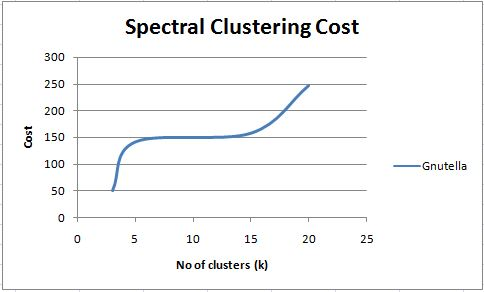
\includegraphics[width=5cm]{spectral_kvscost}}}%
		\end{figure}
		
		
	\item	Since visualizing million nodes with their respective clusters was daunting, we have shown the visualization produced when spectral clustering was run on the \textbf{GNutella} dataset. For k=3 clusters, the visulalization clealry depicts the cluster centers to which each node belongs to.
		
		\begin{figure}[H]%
			\centering
			\subfloat[ Spectral Clustering on Nutella dataset(6401 nodes) for k=3]{{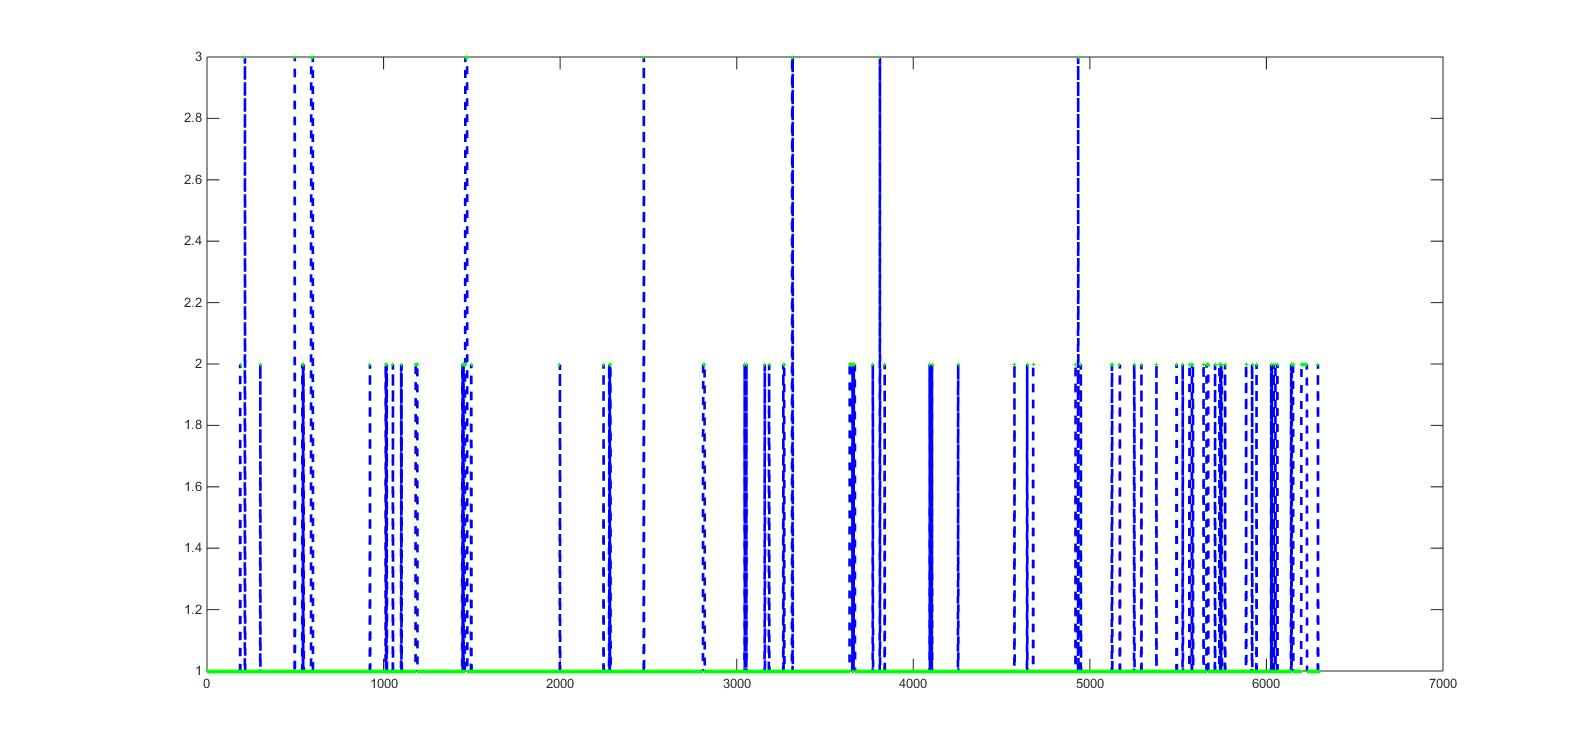
\includegraphics[width=5cm]{Gnutella_Spectral_k3} }}%
			\end{figure}
		
		\item[] \textbf{\underline{Performance comparison between Normalized and Unnormalized Laplacian}}
		
		\textbf{We found that the un normalized Laplacian scaled well with bigger networks whereas the normalized Laplacian encountered "Out of Memory" errors.}The definition of bigger networks here implies networks having more than million edges.
		
		\textbf{For smaller datasets however, normalized Laplacian performed better} and the sparse adjacency matrix which was created had a good distribution which would eventutally lead to a good clustering and smaller costs. The visualization of adjacency matrices for a smaller dataset of 6300 nodes is shown below:
		
		
		\begin{figure}[H]%
			\centering
			\subfloat[Unnormalized :Laplacian-  Spectral Clustering on Nutella dataset]{{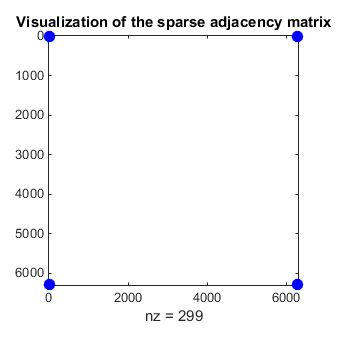
\includegraphics[width=5cm]{random_unnormalized} }}%
			\qquad
			\subfloat[Normalized :Laplacian-  Spectral Clustering on Nutella dataset ]{{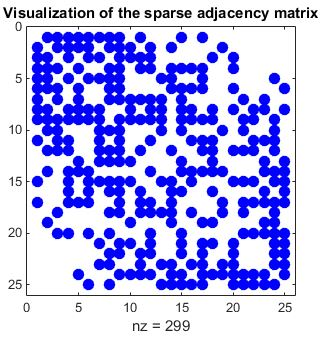
\includegraphics[width=5cm]{adjacency_random_normalized} }}%
		\end{figure}
		
		Clearly the sparse matrix produced by Normalized Laplacian
		would help us put all the vertices on a single line and would give us a better clustering than the unnormalized for smaller datasets.
		
		\subsubsection{Lessons learnt}
		
		\begin{itemize}
			\item Spectral clustering works really well for graph networks and is ideally suitable technique for such network datasets.
			
			\item Scalability, cost function and the execution time values are good indicators of the performance of the spectral clustering.
			
			\item As we increase the \emph{k} value, the value of the cost for partitioning increases and this is due to the fact that it is a top down clustering and as we go down we will make more and more partitions.
			
			\item Eigen structure of the similarity matrix to partition points works well for unnormalized Laplacian and graph networks geometry makes Spectral clustering a good clustering technique.
		\end{itemize}
		
	\end{itemize}
		


\subsection{ K-means clustering}

\begin{itemize}
	
	\item [] The second clustering technique which we tried to explore for our given problem was K-means clustering. It is an assignment based clustering technique and given the number of clusters to be formed it gives us information about which clusters will our data point belong to.
	
	\item[] Again the notion of groups in social network implies similar interests between the people in the network and our clustering would help us find them. \\
	
	\textbf{\underline{Programming Platform Used:  Spark-Scala}}
	
	\subsubsection{Data Storage}
	\begin{itemize}
		\item 
		Again while dealing with such large datasets, storage of data becomes top priority. 
		We first stored the node and it's corresponding edges information. 
		
		\item We imported Vector from linear algebra module to help us store the edges information for each node. The vectors for each node was compared with Hamming Distance as the parameter.
		
		\item Based on this we would know which nodes get clustered together. We can find a node which is the farthest from its present central node and the farthest of these two nodes can be the new cluster center. Now the nodes of the existing clusters, might be closer to the newly designated center and we group such nodes to form a new cluster. This process goes on till we have the required number of clusters.
	\end{itemize}
	
	\subsubsection{ Expectation on the clustering produced}
	\begin{itemize}
		\item We were expecting the KMeans algorithm to pick those nodes as clusters center which are spatially in the center of the  cluster as well. 
		
		\item It is hard to analyse which nodes are probably the most highly connected but we were interested to see if we find some clusters more dense than others which would mean the nodes in that cluster are highly connected.
		
		\item We also wanted the cost, Within-cluster sum of squares to get optimized with increased number of clusters. The assignment and update steps of the algorithm are expected to improve cost.  
		
	\end{itemize}
	
	
	\subsubsection{Basic Approaches tried}	
	\begin{itemize}
		
		\item We worked on KMeans algorithm with the fundamentals we had learnt during our coursework. We randomly initialized the central nodes for the algorithm.
		
		\item Due to the size of our dataset we had problems implementing our algorithm on traditional programming platforms like Matlab and others. Even though Python is a powerful language, again we ran into scalability issues and hence we decided to explore Parallel distribution platforms like Spark.
		
		\item Spark proved to be very effective and scaled well for datasets of all sizes. Spark internally splits our dataset into multiple partitions and multiple operators work together on the same partition of data and hence this optimizes the graph and is the key for Sparks performance. 
		
		\item We wanted to see if the number of clusters,k that our data gets divided into will affect the time component to change. But we inferred that the computation time for our algorithm did not change much with changing number of clusters.
		
		\item We also wanted to optimize our cost, Within cluster sum of squares. This is basically the distance of each node to its nearest center node. We could observe an improvement in this cost with the increasing number of clusters. This makes sense since as the number of clusters increase chances are the points will usually find a cluster center which is closer to it than the previous one.
		
	\end{itemize}	
	
	Having learnt from our initial experiments, the final KMeans algorithm is implemented as provided below:
	
	\subsubsection{Algorithm followed for KMeans Clustering}
	
	\begin{itemize}
		
		\item[]
		1. Initialized cluster centers by randomly picking $k$ nodes from data set.
		
		2. Next we compute the closest center for each node by using map function in Spark which takes each data point in our data set and  finds the center that is closest to it.
		
		3. Once we have found the centers and the nodes close to these centers, we now find the new center by computing the mean of the nodes that are in a single cluster. This is done to each node in a cluster.
		4. Now we again group the nodes based on the cluster center that is closest to them.
		
		5. We continue the above steps until we have the required $k$ number of clusters and cluster centers which happens when the distance between the nodes and their present closest center is lesser than the previous center.
		
	\end{itemize}
	
	\subsubsection{ Results and observations}	
	
	\begin{itemize}
		
		\item[] We wanted to visualize the clusters obtained at the end of the algorithm. We set $k=4$ and tried plotting the LiveJournal data set values. The file turned out to be huge and hence we decided to experiment with smaller datasets with similar structure like dblp and Gnutella network datasets. \\
		As in our dataset finding distance is difficult, we have clustered data points and while plotting the graph, we decided the range and plotted the points for better visualization of clusters. The graph shown below is a scaled-down version of the original output we got from K-means clustering algorithm. In the following dense plot it can be seen that cluster 2 represented by green color is highly connected than the other clusters and for the simulated dataset cluseter 0 represented by red color is highly connected than the other clusters.
		
		We ran the algorithm for medium size datasets and plotted runtime of the algorithm across dblp, Gnutella, simulated dataset and liveJournal. As LiveJournal has millions of nodes and edges, KMeans took more time as compared to other datasets. We also plotted KMeans clustering cost over number of clusters for Dblp dataset which can be seen below. From the pot, we observed that as number of clusters increase, Kmeans cost decreases because number of cluster centers are increased and it in turn decreases distance between datapoints and cluster centers.
	\end{itemize}
	
		\begin{figure}[H]%
			\centering
			\subfloat[KMeans on Gnutella]{{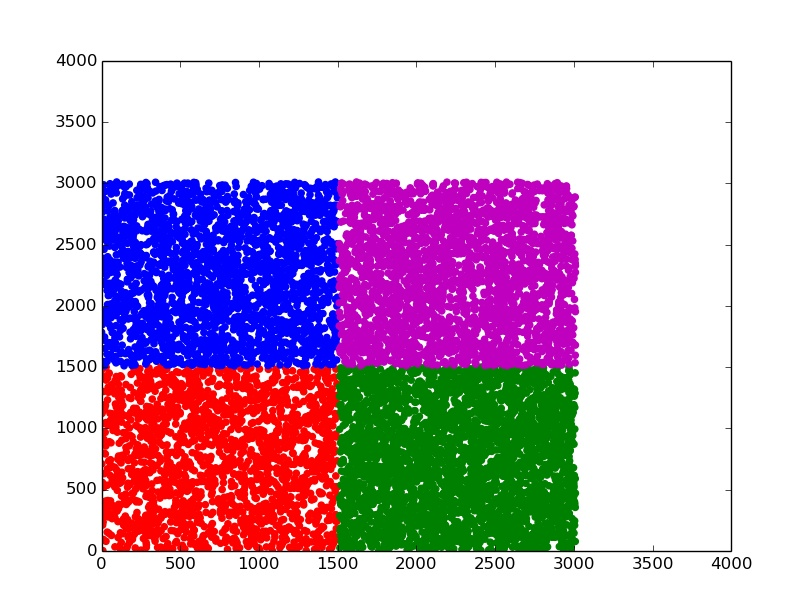
\includegraphics[width=5cm]{dblp_kmeans.jpeg} }}%
			\qquad
			\subfloat[ KMeans on simulated dataset ]{{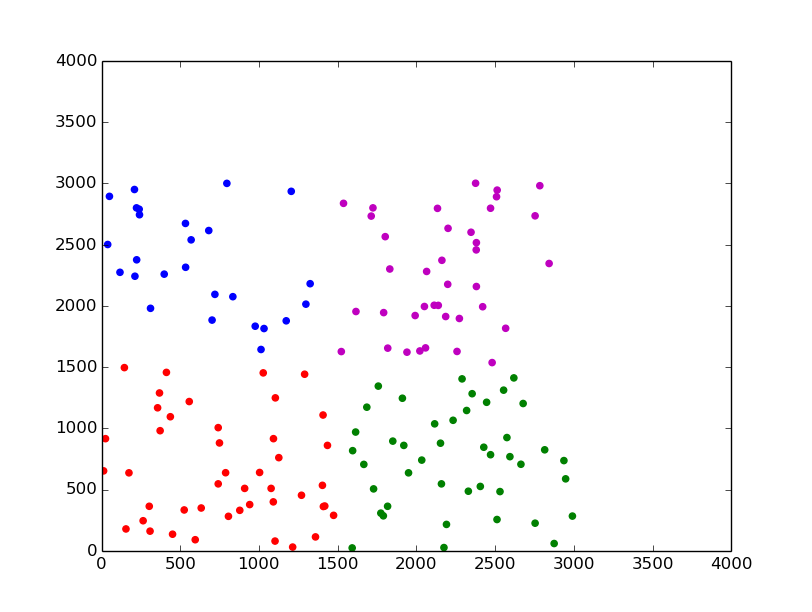
\includegraphics[width=5cm]{Random_kmeans} }}%
			\end{figure}
	
	
	\begin{figure}[H]%
		\centering
			\subfloat[K vs cost for K-Means Clustering ]{{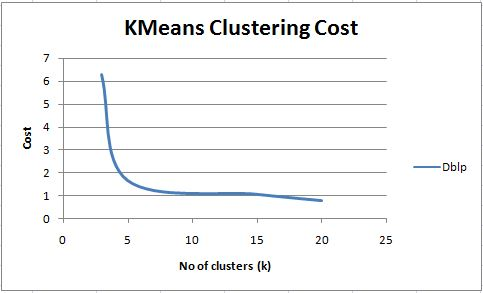
\includegraphics[width=5cm]{k_vs_cost} }}%
		\qquad
		\subfloat[Runtime comparison of different datasets ]{{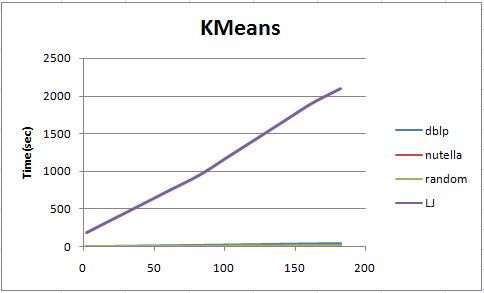
\includegraphics[width=5cm]{Kmeans_time.JPG} }}%
	\end{figure}
	
\end{itemize}
%\end{itemize}


\subsection{ Hierarchical clustering}

 \begin{itemize}
 	\item[] 

The next clustering technique which we tried out on our dataset was Hierarchical or Agglomerative clustering.\\
It is a bottom up style of clustering where we start with very small clusters and then build big clusters. In other words we start with each point as individual clusters and then group them together to form one single cluster.\\

In our data, this would be equivalent to users being individual users before they join the live journal community and once they join and then they join the community they could be part of groups and several groups can combine which will give us one single group comprising of all the users.

\textbf{\underline{Programming Platform Used:  MATLAB}} 
	
	\subsubsection{Data Storage}
	\begin{itemize}
		\item[] Data storage for hierarchical clustering was exactly the same as the one which was followed for spectral clustering and adjacency matrices were created to load the data.
	\end{itemize}
	\subsubsection{Selection of distance Measure}
	\begin{itemize}
		\item Since our dataset is network/graph dataset, the notion of Euclidean distance is not relevant. Hence we decided to use "Hamming distance" as the distance measure for similarity.
		The distance measure used in our code was : \\
		$d^{HAD}(i,j)=\sum_{k=0}^{n-1}[y_{i,k} \neq y_{j,k}]$ 
		
		where, $d^{HAD}$ is the Hamming distance between rows of our Adjacency Matrix.
		
		\item The vectors required for finding Hamming distance between two vectors are obtained from taking the corresponding row of the node in the adjacency matrix.
		\item The mean-link variant of hierarchical clustering was used for the implementation as it is best suited when the dataset size is huge.
	\end{itemize}
	
	\subsubsection{Algorithm for Hierarchical Clustering }
	\begin{itemize}
		\item[] 1. Construct the adjacency matrix for the given undirected graph. For larger datasets, use sparse adjacency matrix for better scalability.
		\item[] 2. Compute the Hamming distances between clusters which are close enough. 
		\item[] 3. Use mean link variant as the linkage formulation for joining the clusters.
		\item[] 4. Find the closest distance between two clusters and merge them into single cluster
		\item[] 5. Stop joining the clusters when you have reached the desired k clusters.
	\end{itemize}

	\subsubsection{Results and observation}
	\begin{itemize}
		\item The Hierarchical clustering algorithm was working well for smaller sized datasets as described in section 4.4. The clusters produced by the Hierarchical Clustering were visualized using a Dendogram and it is shown below:
		
		 \begin{figure}[H]%
		 	\centering
		 	\subfloat[Hierarchical clustering on dataset having 6300 nodes]{{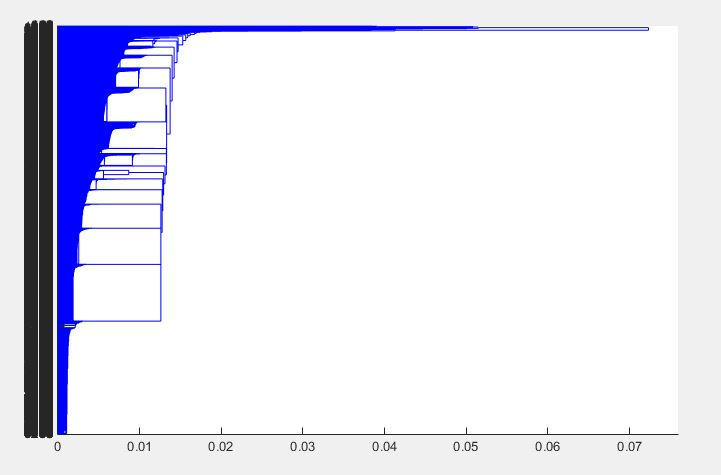
\includegraphics[width=5cm]{gnutella_hierarchical} }}%
		 	\qquad
		 	\subfloat[Hierarchical clustering on dataset having 25 nodes ]{{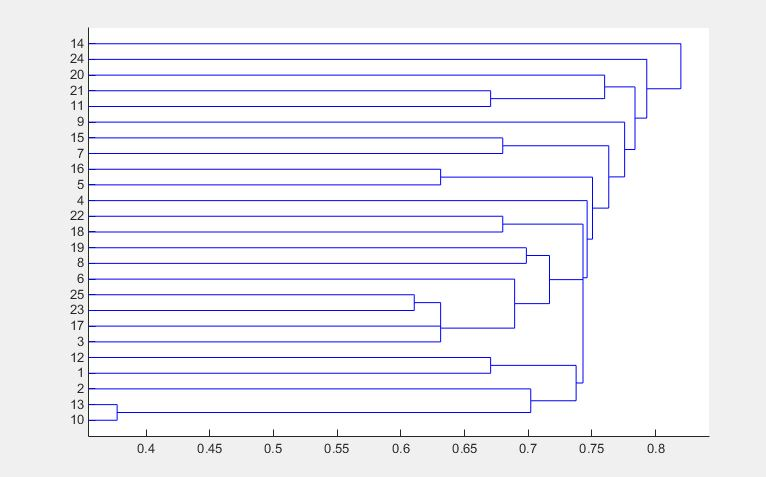
\includegraphics[width=5cm]{nodes25_hierarchical} }}%
		 \end{figure}
	
	The execution times were also noted and the plot below shows the execution times for two different data sets. Larger the size of the dataset,the longer the running time.
	

	\begin{figure}[H]%
		\centering
		\subfloat[Running time comparison for Hierarchical clustering]{{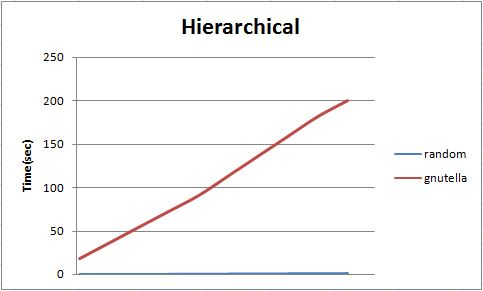
\includegraphics[width=5cm]{Hierarchical_time} }}%
		 \end{figure}

	

\item \textbf{However our Hierarchical clustering algorithm could not scale for medium sized datasets and larger datasets and was failing.} 

\end{itemize}

\subsubsection{Alternative Approaches tried and results observed}

\begin{itemize}
	\item Since there were "Out of Memory" issues, we tried moving to a different programming language and coded it in Python. Instead of fitting in thw whole data set, we tried to split the data set by running k-means algorithm on it.
	\item However the data points in the same clustering were not in the same split after running the k-means and hence we ran into issues as the data  was not correctly separated. We tried to test this approach on a smaller dataset but we encountered problems in re-joining the data and were into a tangle. 
	\item We decided if we could implement this on a cluster set up with Hadoop but we were again not entirely convinced if it our intial split would give us the right results and so didn't proceed further in that direction.
\end{itemize}


\subsubsection{Lessons Learnt}
\begin{itemize}
	\item Hierarchical clustering works well for tiny and smaller datasets.
	\item It does not scale well for bigger datasets and would require pre-processing and running other algorithms, which kind of indicates that this might not be the best technique for the network datasets.
	\item The scalability issue arises due to the fact that the distance computation between all pairs of nodes would require storing values in a nX n matrix or arrray and as n approaches million, MATLAB and programming platforms can't handle such data.
	\item Splitting the huge dataset into smaller chunks and then joining them back again could be one way of implementing hierarchical clustering for large network datasets.
\end{itemize}

 \end{itemize}
\section{ Comparing of clustering techniques on network datasets}


\section{ Other Interesting information mined from our data}

\begin{itemize}
	

\item[] The failure of hierarchical clustering for large datasets made us take a closer look at methods for processing huge datasets on Hadoop and Spark platforms.The quest of finding it coincided with the concept of PageRank introduced in the class lectures. 

\item[] The lack of extra features or details in our dataset didn't deter us from performing further mining on our data. Given that our data represents an actual social network, we decided to find the top k-people who were highly connected or who had the most friends in the network.

\textbf{Method used for finding the highly connected k-people in the network}
\begin{itemize}
	\item[] 1. Split the input large dataset into separate files.
	\item[] 2. Process the individual files and find the out degree of each of the nodes store just the node and its out-degree information.
	\item[] 3. Combine the individual files together and then sort the merged file in descending order of outdegree.
	\item[] 4. Return the top k-people in the network.
\end{itemize}

\item[] The information returned is potentially related to real world scenario. For instance if we were interested in finding the "Most Influential Person" in a network like LinkedIn, this could give us the result. This is potentially a useful information which could be tapped in by different companies or businesses for exapnding their avenues.It could also be used for several different things.

\item[] Apart from finding the highly connected k-people, we also found out the most densely connected or influential person in a network based on his outdegree as well as the importance or weight of the outdegree of his/her neighbouring nodes. The neighbors which are more important contribute more when compared to the large number of neighbors which lie far away and are relatively less important. The visualizations are shown below:

\begin{figure}[H]%
	\centering
	\subfloat[Highly connected k-nodes in a network]{{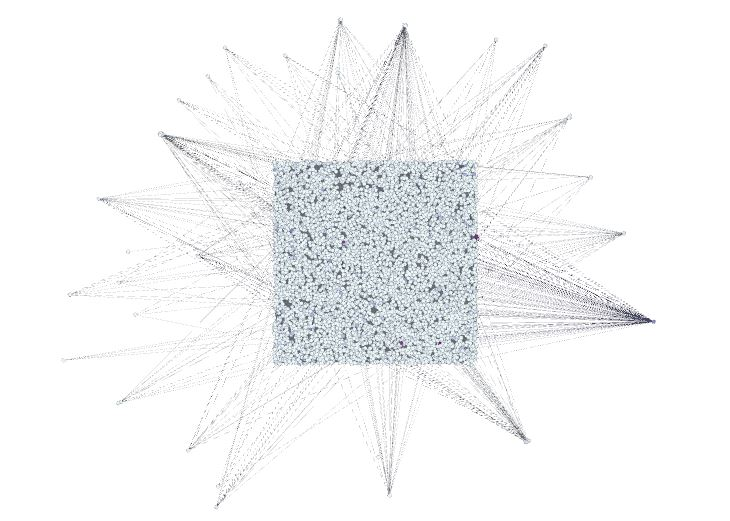
\includegraphics[width=5cm]{dblp2_outdegree_viz} }}%
	\qquad
	\subfloat[Most connected or influential node in a network and its neighbors ]{{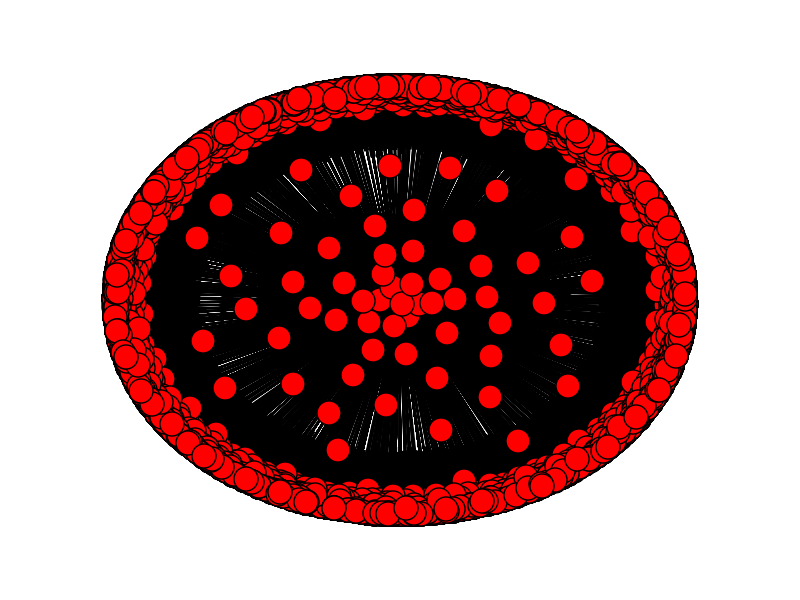
\includegraphics[width=5cm]{Top_rank} }}%
\end{figure}

The visualization on the left was produced by making use of \textbf{Gephi} and the one on the right was produced using Python networkx and draw graph packages. These visualizations were produced by running the code on our main dataset.

\end{itemize}


\bibliographystyle{plain}
\begin{thebibliography}{100}
	\bibitem{one} J�r�ome Kunegis, Ernesto W. De Luca, and Sahin Albayrak. 2010. The link prediction problem in bipartite networks. In Proceedings of the Computational intelligence for knowledge-based systems design, and 13th international conference on Information processing and management of uncertainty (IPMU'10), Eyke H?llermeier, Rudolf Kruse, and Frank Hoffmann (Eds.). Springer-Verlag, Berlin, Heidelberg, 380-389.
	
	
\end{thebibliography}


\end{document}
